\documentclass[a4paper,10pt]{article}
\usepackage[utf8]{inputenc}
\usepackage{hyperref}
\usepackage{graphicx}
\DeclareGraphicsExtensions{.pdf}
\usepackage{fancyhdr}


\usepackage[top=1cm,bottom=1cm,left=2cm,right=2cm,includehead,head=2.5cm,headsep=0.499cm,includefoot,foot=12pt,footskip=2.8cm]{geometry}



% Pages styles
\fancypagestyle{Title}{\fancyhf{}
  \fancyhead[RO]{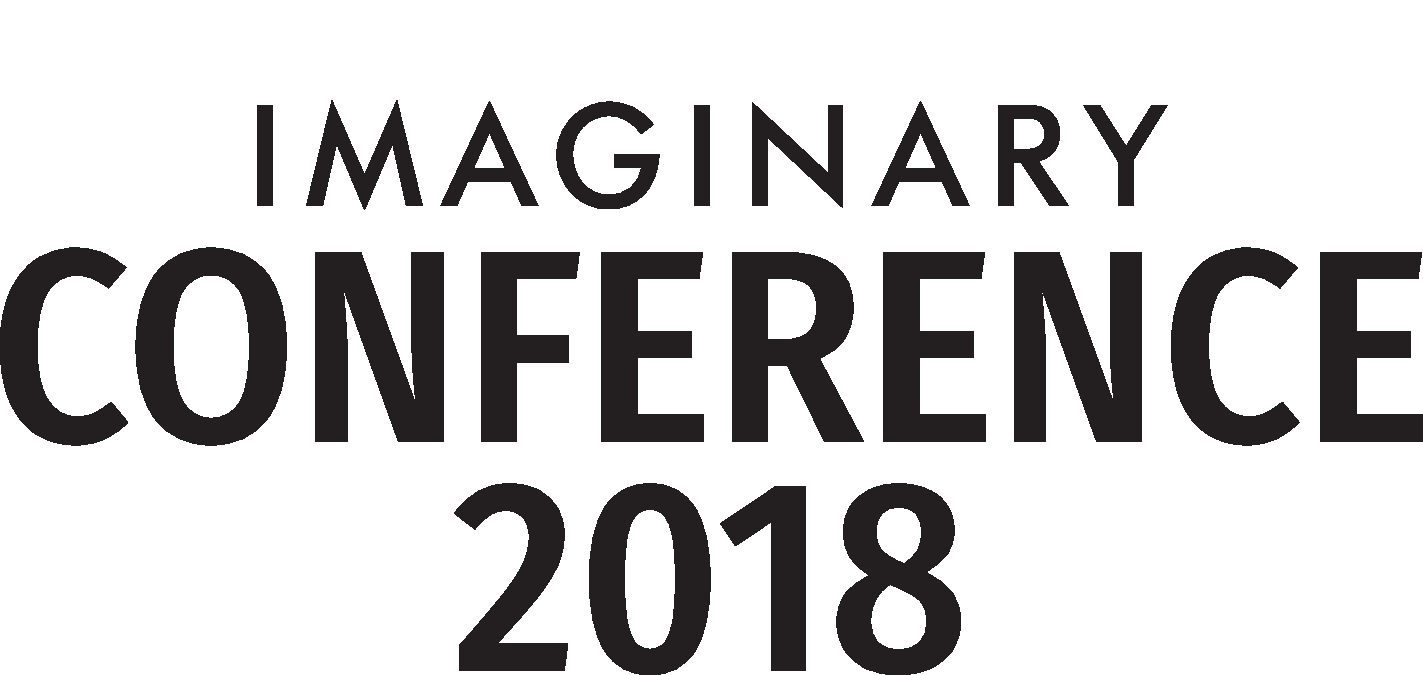
\includegraphics[width=5cm]{IC18-Logo-darkblue.pdf}}
 \renewcommand\headrulewidth{0pt}
}



% Title Page
\title{RPolyhedra: Experiences and beyond}
\author{Alejandro Baranek and Leonardo Belen}

\begin{document}

\maketitle
\thispagestyle{Title} 


\begin{abstract}
An R based library to explore and manipulate Polyhedra from different sources, with OpenGL rendering capabilities. Experiences compiling the library and taking it to the real life.  
\end{abstract}


\section{Information about the speakers}

\subsection{Personal Data}
BARANEK, Alejandro \\
Statistics Specialist \\
BELEN, Leonardo \\
Business Administration Specialist \\

\textbf{Address}: 2233 Rodriguez st., Buenos Aires, Argentina \\
\textbf{Tels.}: +54 (911) 6030 4529/+54 (911) 6106-7032\\
\textbf{Web}: https://qbotics.shinyapps.io/rpolyhedra-explorer \\



\subsection{Speaker information for the conference program}

%Please add a short description of yourself for our conference program (max. 3 sentences). We appreciate to receive a low-resolution photo of you for the conference website. If you agree, please upload your photo as a separate file in the submission form.

As part of the studies to create new ways to construct space frames, we needed to analyze polyhedra and its properties, but - although we found out that some of the most interesting and open source alternatives were not maintained and relied on formats that are not currently used, which would require an effort to process those files to produce a viable visualization. For example, Netlib's Polyhedra\cite{NETLIB}, by Andrew Hume and Visual Polyhedra\cite{DMCCOOEY} by David McCooey. 

With that in mind, we created a standards based R package, which is available on the CRAN Repository as "Rpolyhedra" and enables users to handle and explore polyhedra with minimum effort. Furthermore, as part of the effort, we also created a web based representation\cite{RPOLY_EXPLORER}.
     

\section{Information about the talk}

\subsection{Talk classification}

%There is no restriction on the topics you can present. However, in case your talk fits within the five general conference topics (see \url{http://ic18.imaginary.org/ for details}), please select it below:
%\begin{itemize}
%\item Visualization, new tools and creation of mathematics exhibits
%\item Community, networking 
%\item Knowledge transfer and pedagogics 
%\item Mathematical writing, journalism and media
%\end{itemize}
\begin{itemize}
\item Visualization, new tools and creation of mathematics exhibits
\item Knowledge transfer and pedagogics 
\end{itemize}

\subsection{Talk overview}
%Describe here the content of your talk: State the main questions you address in your talk, describe the background of these questions and your main ideas. You can write max. 2 pages excluding references.

%Pictures with meaningful relation to your topic are welcome, but not mandatory. If you send us pictures, please give information about its copyright and permissions to publish it on a website, see Figure 1.
A guide through the experience of compiling information from free sources to make a tool that can be used to learn and explore polyhedra in an intuitive way, the lessons learnt and how that can improve the knowledge available to the general public. The compiled library is comprised by over 800 polyhedra from different sources, and can be easily extended to include new libraries, due to the fact that the code to scrape the included sources are shipped with the R package. 

Along with the creation of the library, the talk will continue with our experiences on taking its lessons to the next level, and our experience on Augmented Reality and 3D printing which lead us to the creation of a unique node model that can be used to construct polyhedra out of drinking straws for easy prototyping.  



%\begin{figure}
%  \begin{center}
 %   \includegraphics[width=5cm]{mueller.jpeg}
%  \end{center}
%\caption{Image by Boy M\"uller. (c) Mathematisches Forschungsinstitut Oberwolfach}
%\end{figure}


\bibliographystyle{plain}

\begin{thebibliography}{10}
\bibitem{NETLIB}{Polyhedra. HUME, Andrew and others. http://www.netlib.org/polyhedra/}
\bibitem{DMCCOOEY}{Visual Polyhedra, MCCOOEY, David, http://dmccooey.com/polyhedra/}
\bibitem{RPOLY_EXPLORER}{Polyhedra Explorer, BARANEK, Alejandro and BELEN, Leonardo, https://qbotics.shinyapps.io/rpolyhedra-explorer/}
\end{thebibliography}


%\section{How to name and upload of this document (CUT AWAY!) } 

%\textit{please delete this section before you submit your proposal}

%\paragraph{Document name} To make it easier for us to store, find and use your proposal, please stick to the following rules:

%\begin{itemize}
% \item Please call the document as \textit{ic18\textunderscore talk\textunderscore YourSurname.pdf}.
% \item Please use no spaces within the document name
%\end{itemize}

%\paragraph{Submit your proposal}

%To submit your proposal, send the documentation to ic18@imaginary.org
%with the text ``Talk Submission''  in the subject. Please copy your title
%and abstract into the body of the email and attach your complete
%proposal as one pdf document. 


%\paragraph{Submission deadline}
%The deadline for proposal submission is
%August 15th, 2018. We strongly encourage you to submit your proposal as
%early as possible (though the decision of the scientific committee does
%not depend on your submission date).  



\end{document}          
